\chapter{Unemployment Insurance}

\fancyhead[L]{ECON0024}
\fancyhead[C]{Ch.1 Unemployment Insurance}
\fancyhead[R]{Xiaotian Tian}
\fancyfoot[L]{\hyperlink{tableofcontents}{Back to Table of Contents}}
\fancyfoot[R]{Xiaotian Tian}

\section{Unemployment}

    \subsection{Definition of Unemployment}
        The International Labour Organisation (ILO)'s \emphb{definition of unemployment}: The number of jobless people who want to work, are available to work, and are actively seeking employment
        
    \subsection{Why we care about unemployment?}
        \begin{enumerate}
            \item Unemployment is a sign of \emphb{inefficiency}.
            \item Modern view: part of the unemployment arises from \emphb{search costs (or frictions)}.
                \begin{itemize}
                    \item Zero unemployment is sub-optimal, because it indicates intensive job searching that induces high search costs.
                    \item Therefore, some level of unemployment (usually 3\% - 6\%) are tolerated in reality
                \end{itemize}
            \item Being unemployed decreases life satisfaction.
        \end{enumerate}

\section{Introduction to Unemployment Insurance (UI)}

    \subsection{Introduction}
        Many countries have some kind of UI, but it still remains controversial due to its benefit-and-cost \emphb{tradeoff}:
        \begin{itemize}
            \item Main benefit: helps people in a time of need
            \item Main cost: reduces incentive to search for work while unemployed
        \end{itemize}
        The following section will analyse how to design unemployment insurance given this trade-off.
        
    \subsection{Brief History of Unemployment Insurance}
        \begin{itemize}
            \item The first unemployment benefit scheme was introduced in the UK with the \textit{National Insurance Act} in 1911.
            \item U.S. introduced UI in 1935 in response to the Great Depression.
            \item Most European countries introduced UI after the WWII during the expansion of welfare state.
            \item Today, most developed countries have some UI schemes.
        \end{itemize}
        
    \subsection{Institutional Details}
        Typically, UI is financed through a payroll tax on employers and/or employees, but the incidence and rates vary a lot across countries. In exchange of the paid in contributions, unemployment benefit are received upon job-loss.
        \begin{itemize}
            \item Usually, the eligibility for UI must be a result of a layoff.
            \item The length and the level of UI benefits often depend on the amount and time length of contribution.
            \item Minimum contribution period and minimum contribution amount are often defined.
            \item The relationship between contribution and benefit-level is often highly non-linear (benefit caps, minimum benefits).
        \end{itemize}
        
    \subsection{Net Benefit Replacement Rate}
        We define the \emphb{Net Benefit Replacement Rate}, an important feature of UI, as:
        $$\text{Net\ Benefit\ Replacement\ Rate} = \frac{\text{Weekly\ Benefit}}{\text{Weekly\ Wage\ Earnings}}$$
        
\section{$\star$ Optimal Unemployment Insurance with No Moral Hazard}

    \subsection{Expected Utility Model of Unemployment}
        A typical objective considered by economists is to maximize agents' welfare given by expected utility.
        
        Specifically, we can calculate the \emphb{expected utility} by:
        $$E[U] = (1-p)\times{U(c^e)} + p\times{U(c^u)} - \psi(1-p)$$
        where
        \begin{itemize}
            \item $p$ is the probability of being \emph{unemployed} ("unemployment rate")
            \item $1-p$ is the probability of being \emph{employed}
            \item $c^u$ is the consumption when being \emph{unemployed}
            \item $c^e$ is the consumption when being \emph{employed}
            \item $U(.)$ is the utility function: we assume it to be \emph{strictly increasing and concave} i.e. $U'(.)>0$ and $U''(.)<0$
            \item $\psi(.)$ is the job searching cost function: we assume it to be \emph{strictly increasing and convex} i.e. $\psi'(.)>0$ and $\psi''(.)>0$
        \end{itemize}
        
            \subsubsection{Assumptions on the individual side}
                Assume \emphb{no saving/borrowing} and \emphb{homogeneous agents}:
                \begin{itemize}
                    \item Consumption at employment equals to after-tax wage i.e. $c^e = w-t$
                    \item Consumption at unemployment equals to UI benefit i.e. $c^u = b$
                \end{itemize}
                With this assumption, we can express the \emph{expected utility} as:
                \begin{equation}
                    E[U] = (1-p)\times{U(w-t)} + p\times{U(b)} - \psi(1-p)
                    \label{eqn:ui_exp_utility}
                \end{equation}
                
            \subsubsection{Assumptions on the government side:}
                Assume that the government must have a \emphb{balanced budget}: total tax collected must equal to total benefit given. With this assumption, we can write the government's \emphb{budget constraint}:
                $$(1-p)\times{t} = p\times{b}$$
                Rearranging this equation, it indicates that taxes need to be:
                $$t = \frac{p}{1-p}\times{b}$$
                plug these results into the expected utility of individuals (equation \ref{eqn:ui_exp_utility}):
                $$E[U] = (1-p)\times{U(w-\frac{p}{1-p}\times{b})} + p\times{U(b)} - \psi(1-p)$$
                Therefore, we can express the \emphb{government's optimisation problem} as:
                \begin{equation}
                    \label{eqn:ui_no_mh}
                    \max_{b} E[U] = (1-p)\times{U(w-\frac{p}{1-p}\times{b})} + p\times{U(b)} - \psi(1-p)
                    \end{equation}
                    
            \subsubsection{Further assumption: No moral hazard}
                Assume that $p$, the probability of finding a job, does not depend on the benefit level $b$, i.e. \emphb{no moral hazard}. We can treat $p$ as an exogenous variable here.
                
                \emph{Reminder: here, moral hazard refers to the adverse actions taken by insured individuals in response to insurance against adverse outcomes. It exists as long as insurers cannot perfectly monitor insurees.}
                
        \subsection{Optimisation Result: Full Insurance}
            To find the optimal UI, we solve the optimisation problem (\ref{eqn:ui_no_mh}). The FOC is:
            $$\frac{\partial E[U]}{\partial b}=-(1-p)\times{\frac{p}{1-p}}\times{U'(w-\frac{p}{1-p}\times{b})} + p\times{U'(b)} = 0$$
            $$U'(b) = U'(w-\frac{p}{1-p}\times{b})$$
            $$\color{red} b = w-\frac{p}{1-p}\times{b}$$
            This result implies that
            \[\color{red} c^e = w-t = b = c^u\]
            which indicates \emphb{full insurance} -- people have the same income when unemployed as they were employed. In practice, this would mean that the net replacement rate = 1. (\empha{No moral hazard $\leadsto$ Full insurance})
            
\section{$\star$ Optimal Unemployment Insurance with Moral Hazard}

    \subsection{Moral Hazard}
        The problem with full insurance is that it eliminates incentives to work. To incorporate \emphb{moral hazard} into our framework, we assume that $p$ increases with $b$: more generous benefits deter job search and hence increase unemployment.
        $$p=p(b),\ \frac{\partial p(b)}{\partial b}>0$$
        
    \subsection{Individuals' Response}
        Now, individuals choose their probability of being unemployed $p$ given the unemployment benefit $b$:
        $$\max_p E[U] = (1-p)\times{U(c^e)} + p\times{U(c^u)} - \psi(1-p)$$
        The FOC of this problem is:
        $$\frac{\partial E[U]}{\partial p}=-U(c^e)+E(c^u)+\psi'(1-p) = 0$$
        Manipulate:
        $$Pr(employed) = 1-p = \psi'^{-1}\Big(U(c^e)-U(c^u)\Big)$$
        Note that $c^e, c^u$ are also functions of $b$:
        \begin{equation}
            \label{eqn:ui_mh_optimal_p}
            Pr(employed) = 1-p(b) = \psi'^{-1}\Big(U(w-\frac{p}{1-p}\times{b})-U(b)\Big)
        \end{equation}
        Now, we can investigate the effect of changing $b$ on the probability of being employed (using $\frac{\partial f^{-1}(x)}{\partial x} = \frac{1}{f'(x)}$):
        $$\frac{\partial Pr(employed)}{\partial b}=\frac{\partial(1-p(b))}{\partial b} = \frac{-\frac{p}{1-p}\times{U'\big(w-\frac{p}{1-p}\times{b}\big)}-U'(b)}{\psi''\Big(U\big(w-\frac{p}{1-p}\times{b}\big)-U(b)\Big)} < 0$$
        because $U'(.)>0$ and $\psi''(.)>0$ by assumption.
        
    \subsection{The government's optimisation: Partial Insurance}
        Our model now becomes:
        $$\max_b E[U] = \big(1-p(b)\big)\times{U\left(w-\frac{p(b)}{1-p(b)}\times{b}\right)} + p(b)\times{U(b)} - \psi\big(1-p(b)\big)$$
        The FOC becomes more complicated:
        $$0 = -U'\left( w-\frac{p(b)}{1-p(b)}\times{b} \right)\times{\left(\frac{p'(b)\times{b}}{1-p(b)}+p(b)\right)} + p(b)U'(b) + p'(b)\times\underbrace{\big[-U(c^e)+U(c^u)+\psi'(1-p(b))\big]}_{\text{From\ the\ FOC\ of\ individuals,\ we\ know\ this\ is\ 0}}$$
        $$0 = -U'\left(\underbrace{ w-\frac{p(b)}{1-p(b)}\times{b} }_{c^e}\right)\times{\left(\frac{p'(b)\times{b}}{1-p(b)}+p(b)\right)} + p(b)U'(\underbrace{b}_{c^u})$$
        Rearrange this, we can get the \empha{Main Equation of Optimal UI}:
        \begin{equation}
            \label{eqn:ui_mh_main}
            \color{red}
            \underbrace{\frac{U'(c^u)-U'(c^e)}{U'(c^e)}}_{\text{Insurance\ Value}} = \underbrace{\frac{1}{1-p}\times{\epsilon_{p,b}}}_{\text{Moral\ Hazard\ Cost}}
        \end{equation}
        where $\epsilon_{p,b} = \frac{b}{p}\frac{dp}{db}$ is the \emphb{elasticity of unemployment rate with respect to benefits}.
        
        Note that the Main Equation of Optimal UI implies: if $\epsilon_{p,b}>0$, then $0<c^u<c^e<w$ which means \emphb{partial insurance} will be the optimum. (\empha{Moral hazard $\leadsto$ Partial insurance})
        
    \subsection{Explaining the Main Equation of Optimal UI}
        As in a typical optimum, the marginal benefit (insurance value) has to be equal to the marginal cost (moral hazard cost). If the marginal benefit (insurance value) is larger than the marginal cost (moral hazard cost), we need to increase the UI benefit to reach optimum, v.v.
        \begin{enumerate}
            \item \textbf{\emphb{Insurance Value}}\\
            This is the marginal benefit of UI benefit (redistributing one unit from the employed to the unemployed): if we increase the UI benefit by 1 unit, the net benefit will be the insurance value:
            $$\text{Insurance\ Value} = \frac{U'(c^u)-U'(c^e)}{U'(c^e)}$$
            \item \textbf{\emphb{Moral Hazard Cost}}\\
            This is the marginal cost of UI benefit (redistributing one unit from the employed to the unemployed): if we want to increase the UI benefit by 1 unit, we need to collect an extra of: $p(b) + p'(b)\times b$. This has to be paid by people who remain employed, so the tax rate has to increase by: $\frac{p(b)+p'(b)\times{b}}{1-p(b)}$. Rearrange:
            $$\text{Moral\ Hazard\ Cost} = \frac{p(b)}{1-p(b)}\times\left(1+p'(b)\times\frac{b}{p(b)}\right) = \frac{p(b)}{1-p(b)}\times(1+\epsilon_{p,b})$$
            This can be understood as the extra cost imposed on an employed individual in order to redistribute 1 unit to every unemployed individual. The more responsive the unemployment rate is (higher $\epsilon_{p,b}$), the more costly of an increase in UI will be.
        \end{enumerate}
        
    \subsection{Sufficient Statistic Approach}
    
        \subsubsection{Approximate the Main Equation of Optimal UI}
            The term $\frac{U'(c^u)-U'(c^e)}{U'(c^e)}$ cannot be estimated because people's utility functions are not observed. Instead, we employ the 1st order Taylor Expansion. Expand $U'(c^u)$ around $c^e$:
            $$U'(c^u) \approx U'(c^e) + U''(c^e)(c^u-c^e)$$
            Therefore:
            \begin{equation*}
                \begin{split}
                \frac{U'(c^u)-U'(c^e)}{U'(c^e)} & \approx \frac{U'(c^e) + U''(c^e)(c^u-c^e)-U'(c^e)}{U'(c^e)}\\
                & = \frac{U''(c^e)(c^u-c^e)}{U'(c^e)}\\
                & = \underbrace{-\frac{c^e U''(c^e)}{U'(c^e)}}_{\text{Relative\ Risk\ Aversion}\ \gamma} \times \frac{c^e-c^u}{c^e}\\
                & = \gamma \times \frac{c^e-c^u}{c^e}\\
                & = \gamma \times \frac{\Delta c}{c^e}
            \end{split}
            \end{equation*}
            Substituting this into the main equation (\ref{eqn:ui_mh_main}):
            \begin{equation}
            \label{eqn:ui_hm_sufficient}
            \color{red}
                \underbrace{\frac{1}{1-p}\times{\epsilon_{p,b}}}_{\text{Moral\ Hazard\ Cost}} \approx \underbrace{\gamma \times \frac{\Delta c}{c^e}}_{\text{Insurance\ Value}}
            \end{equation}
            This equation (\ref{eqn:ui_hm_sufficient}) is a transformation of the Main Equation of Optimal UI, which is estimable in practice:
            \begin{itemize}
                \item $\frac{\Delta c}{c^e}$ is the consumption drop at unemployment
                \item $\gamma$ is the coefficient of relative risk aversion (higher RRA indicates more risk aversion)
                \item $\epsilon_{p,b} = \frac{b}{p}\frac{dp}{db}$ is the elasticity of unemployment rate with respect to benefits
            \end{itemize}
            We call this the \emphb{Sufficient Statistic Approach} because the optimal UI can be calculated aftering measuring the above three factors.
            
        \subsubsection{Pros and Cons of the Sufficient Statistic Approach}
            The alternative method of determining the optimal UI benefit is known as the \emphb{structural labour approach}:
            \begin{enumerate}
                \item Estimate the key parameters of the utility function, job search function, etc.
                \item Simulate counterfactual results with alternative levels of the UI benefit
            \end{enumerate}
            The first procedure often requires functional assumptions on the utility function and the cost of job search. Compared with this, the Sufficient Statistic Approach focus on some key statistics without identifying the whole model of job search. Thus, it has obvious pros and cons:
            \begin{itemize}
                \item \textbf{Key advantage}: easier to implement and less assumptions are needed
                \item \textbf{Key disadvantage}: the derivation of the Main Equation of Optimal UI depends critically on the \emph{envelop theorem} which only holds for small policy deviations (and we used the 1st order Taylor Expansion, which is a local approximation), so it cannot be used to assess the impact of radical changes
            \end{itemize}

\section{Estimation of Moral Hazard ($\epsilon_{p,b}$)}
    Moral hazard in UI is thought to manifest itself in the duration of unemployment: economists investigate whether unemployed individuals find jobs more slowly when UI benefits are higher. The key challenge is to use quasi-experiments to identify these effects.
    
    \subsection{Difference-in-Difference}
        The idea is to exploit changes in UI laws that affect a \emph{treatment} group and compare that with a \emph{control} group.
        \begin{figure}[h]
            \centering
            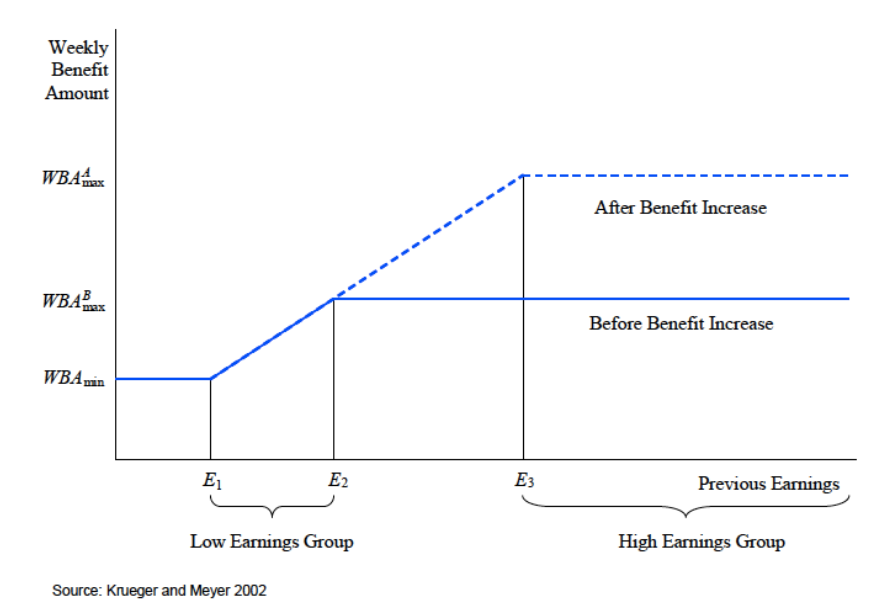
\includegraphics[width=4 in]{images/ch1/did_1.png}
            \caption{Example of DiD: low earnings group as control and high earnings group as treatment}
        \end{figure}
        \begin{enumerate}
            \item Standard DiD specification with 2 states and 2 time period
            $$log(Unemployment\ Duration)_{ist} = \beta_0 + \beta_1 After_{ist} + \beta_2 Treat_{ist} + \beta_3 Treat_{ist} \times After_{ist} + \epsilon_{ist}$$
            where:
            \begin{itemize}
                \item $log(Unemployment\ Duration)_{ist}$ is the log unemployment duration of individual i in state s at time t
                \item $After_{ist}$ is the time dummy
                \item $Treat_{ist}$ is the treatment dummy
            \end{itemize}
            Under the \emphb{Common/Parallel Trend Assumption} (the difference in unemployment duration would have been the same between the treatment/control group in absence of the policy change), $\beta_3$ identifies the casual effect (ATT, specifically).
            \item Fixed Effects Version\\
            $$log(Unemployment\ Duration)_{ist} = \alpha_s + \theta_t + \beta log(b_{ist}) + \gamma X_{ist} + \epsilon_{ist}$$
            where:
            \begin{itemize}
                \item $\alpha_s$ is the state fixed effect
                \item $\theta_t$ is the time fixed effect
                \item $X_{ist}$ includes other control variables
            \end{itemize}
            $\beta$ identifies the relationship between percentage change in replacement rate and percentage change in unemployment duration under FE/FD assumptions. (Correct specification; Random sampling; Time variations and no perfect multicolinearity in regressors; Zero conditional mean)\\
            Meyer (1990) and many other implement this method using data on unemployment duration in the U.S. and state-level reforms. The general finding shows a \empha{benefit elasticity of 0.4-0.6}: 10\% rise in unemployment benefits leads to about a 4-6\% increase in unemployment duration.
        \end{enumerate}
            
    \subsection{Regression Discontinuity Designs}
        This empirical strategy exploits jumps in UI benefits at a threshold.
        \emph{\textbf{Main assumption}}: \emphb{Continuity}: individuals who are slightly below the threshold and individuals who are slightly above the threshold would have similar unemployment duration in absence of the jump in the UI benefit level at the threshold.
        
        This assumption will not hold if:
        \begin{itemize}
            \item There are \emph{selection/manipulation} on one side of the threshold. For example, the unemployed somehow achieve to lay-off a few days to deliberately reach the threshold.
            \item There are other policy changes that affect outcomes at the threshold.
        \end{itemize}
        Example:\\
        Card-Chetty-Weber (2007) used the fact that in Austria, you get up to 30 weeks of benefits when you have been employed for 36+ months in last 5 years (instead of up to 20 weeks).
        \begin{figure}[H]
            \centering
            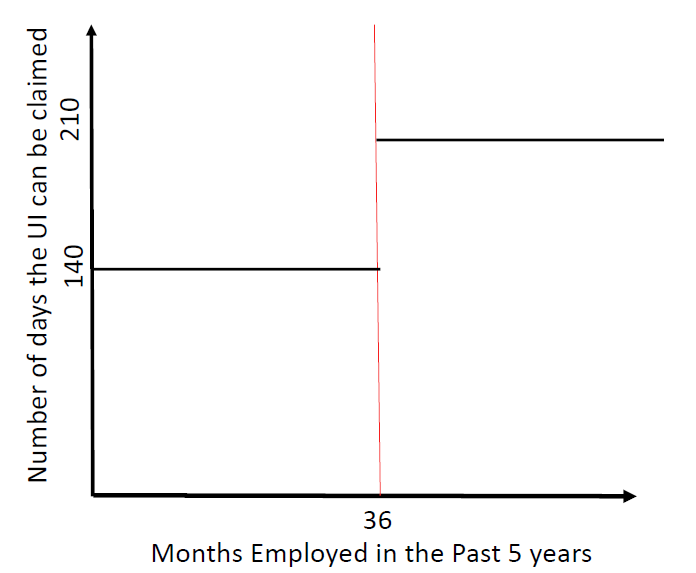
\includegraphics[width=3 in]{images/ch1/card_1.png}
            \caption{Jump in UI Benefit}
            \label{fig:card_1}
        \end{figure}
        They checked: (1) there is no selection around the threshold (on frequency of layoffs, age, wages, etc.) (2) there is no other policy change at the threshold.
        \begin{figure}[H]
            \centering
            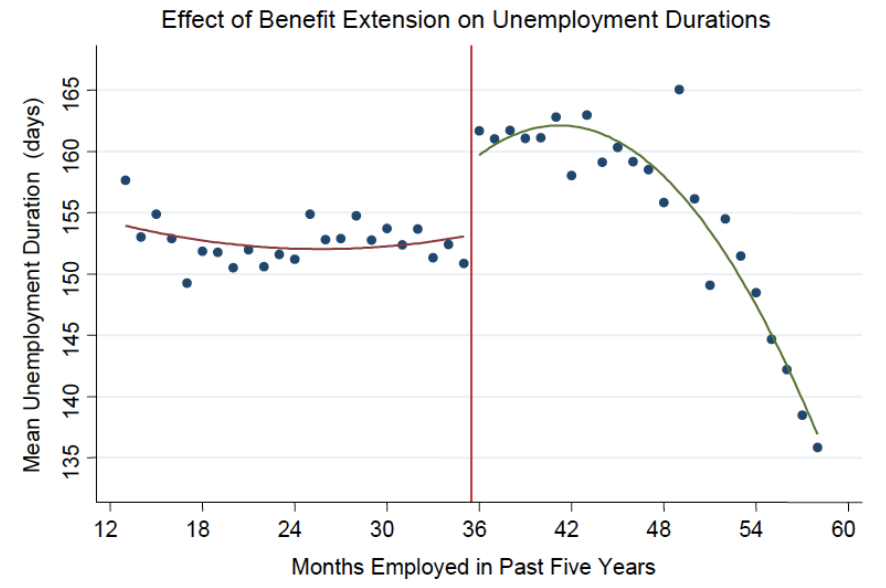
\includegraphics[width=4 in]{images/ch1/card_2.png}
            \caption{RDD Result}
            \label{fig:card_2}
        \end{figure}
        They estimated a benefit elasticity $\epsilon_{p,b} \approx 0.3$.
        
    \subsection{Regression Kink Designs}
        This strategy is very similar to RDD, but we exploit a kink in UI benefits instead of a jump.
        \emph{\textbf{Main assumption}}: In the absence of the kink in the benefit-level, there would be no kink in unemployment duration.\\
        Example:\\
        Kolsrud, Landais, Nilsson and Spinnewijn (2016) studied a kinked UI benefit scheme in Sweden from 1999 to 2000:
        \begin{figure}[H]
            \centering
            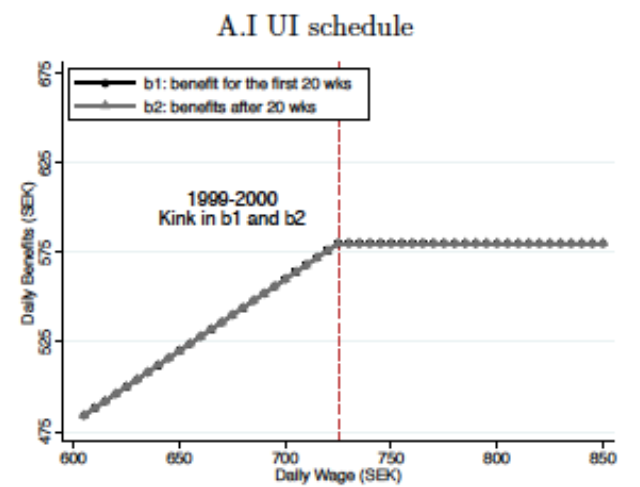
\includegraphics[width = 3 in]{images/ch1/RKD_1.png}
            \caption{Kinked UI Benefits}
            \label{fig:RKD_1}
        \end{figure}
        They found a kink in unemployment duration, indicating the existence of moral hazard:
        \begin{figure}[H]
            \centering
            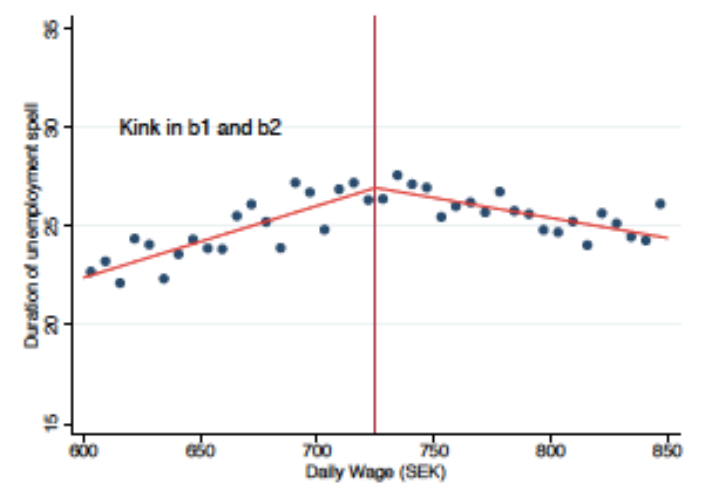
\includegraphics[width = 3 in]{images/ch1/RKD_2.png}
            \caption{Kinked Unemployment Duration}
            \label{fig:RKD_2}
        \end{figure}
        In this case, the assumption can be easily checked: after 2000, the kinked UI benefits was abandoned, and the kink in unemployment duration disappeared:
        \begin{figure}[H]
            \centering
            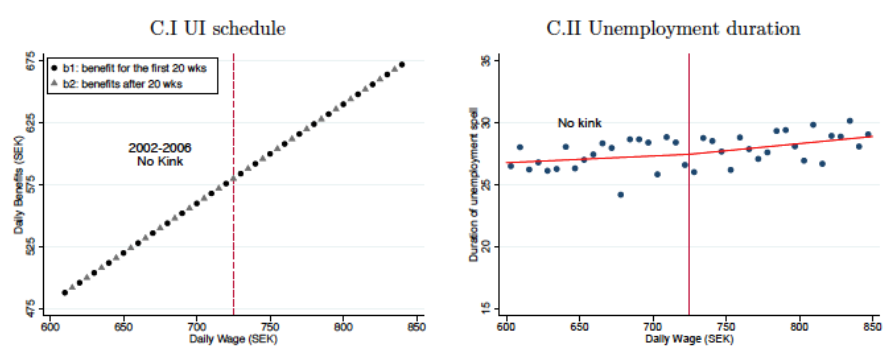
\includegraphics[width = 6 in]{images/ch1/RKD_3.png}
            \caption{Check the Assumption}
            \label{fig:RKD_3}
        \end{figure}
        
        \subsection{Extension: Decompose the Effect Using the Slutsky Equation}
            \subsubsection{Decomposition}
                Similar to the Slutsky Equation, we can decompose the overall effect of changes in UI benefit on job research of the unemployed into a liquidity effect and a moral hazard effect (discussed by Card, Chetty, and Webers (2007)):
                $$\underbrace{\frac{\partial s_t}{\partial b_t}}_{\text{Overall\ Effect}} = \underbrace{\frac{\partial s_t}{\partial A_t}}_{\text{Liquidity\ Effect}} - \underbrace{\frac{\partial s_t}{\partial w_t}}_{\text{Moral\ Hazard\ Effect}}$$
                where:
                \begin{itemize}
                    \item Liquidity Effect shows how search would change if cash was given to the agent independently of being unemployed or not -- giving an extra dollar of UI benefits increases the wealth of the receiver, making them feel "richer."
                    \item Moral Hazard Effect shows the distortion effect of UI benefit -- giving an extra dollar of UI benefit distorts the "price" of being unemployed compared with being employed, i.e. the receiver may have lower incentives to look for a job.
                \end{itemize}
            \subsubsection{Estimation Using Two RDD}
                Card et. al. (2007), estimated the overall effect and liquidity effect, then calculated the moral hazard effect using the above decomposition.
                \begin{itemize}
                    \item Estimating Overall Effect: RDD exploiting the fact that people with less than 36 months of employment in the past 5 years receive 20 rather than 30 weeks of UI. Compare non-employment duration of those just below the 36 months threshold and those just above it.
                    \item Estimating Liquidity Effect: RDD exploiting the fact that firms are forced to pay a lump-sum severance payment equal to 2 months of previous salary to workers who are laid off after 3 years of service. Compare workers who are just below the 3 year cutoff with those just above, and look at the difference in their non-employment duration.
                \end{itemize}
        
\section{Evidence on Consumption Smoothing ($\frac{\Delta c}{c^e}$)}
    The evidence on consumption smoothing is more limited. The key constraint is data: while we have millions of observations of unemployment duration (administrative records), data on consumption is often restricted to surveys, which contain much less samples. (Typically, we need a large sample size to use RDD/RKD.)
    
    \subsection{Difference-in-Difference}
        The settings are similar to the DiD strategy mentioned before. Gruber (1997) used food consumption as the dependent variable, and used cross-state and time variations. The dataset used is PSID food consumption.
        
        Gruber identified the following equation:
        $$\frac{\Delta c}{c^e} = \beta_0 + \beta_1 \frac{b}{w_i}$$
        
        Their results show that: $\beta_0 \approx 0.24$ and $\beta_1 \approx -0.28$. Without UI benefits, unemployment will cause a 24\% drop in consumption. With the current level of UI benefit (net benefit replacement rate $\frac{b}{w_i}=0.5$), the consumption is estimated to drop about 10\%, and a 10\% increase in UI benefits will induce a 2.8\% reduction in the consumption drop.
        
        This provides convincing evidence that insurance markets are not perfect and UI does play a consumption smoothing role.
        
        Note that the drop in benefit-level and the drop in consumption is much less than 1-1. This is because UI also affects people's \emphb{Self Insurance} behaviour:
        \begin{itemize}
            \item Saving behaviours
            \item Spousal labor supply
            \item Borrowing from friends
        \end{itemize}
        Provision of UI benefits crowds out such self insurance to some extent.
    
    \subsection{Using Data of Bank Accounts}
    
        Ganong (2016) uses JPMorgan Chase Institute’s (JPMCI) data on anonymized data on 210,000 checking accounts that received a direct deposit of unemployment insurance (UI) benefits. This overcomes the small sample problem present in survey data.
        \begin{figure}[H]
            \centering
            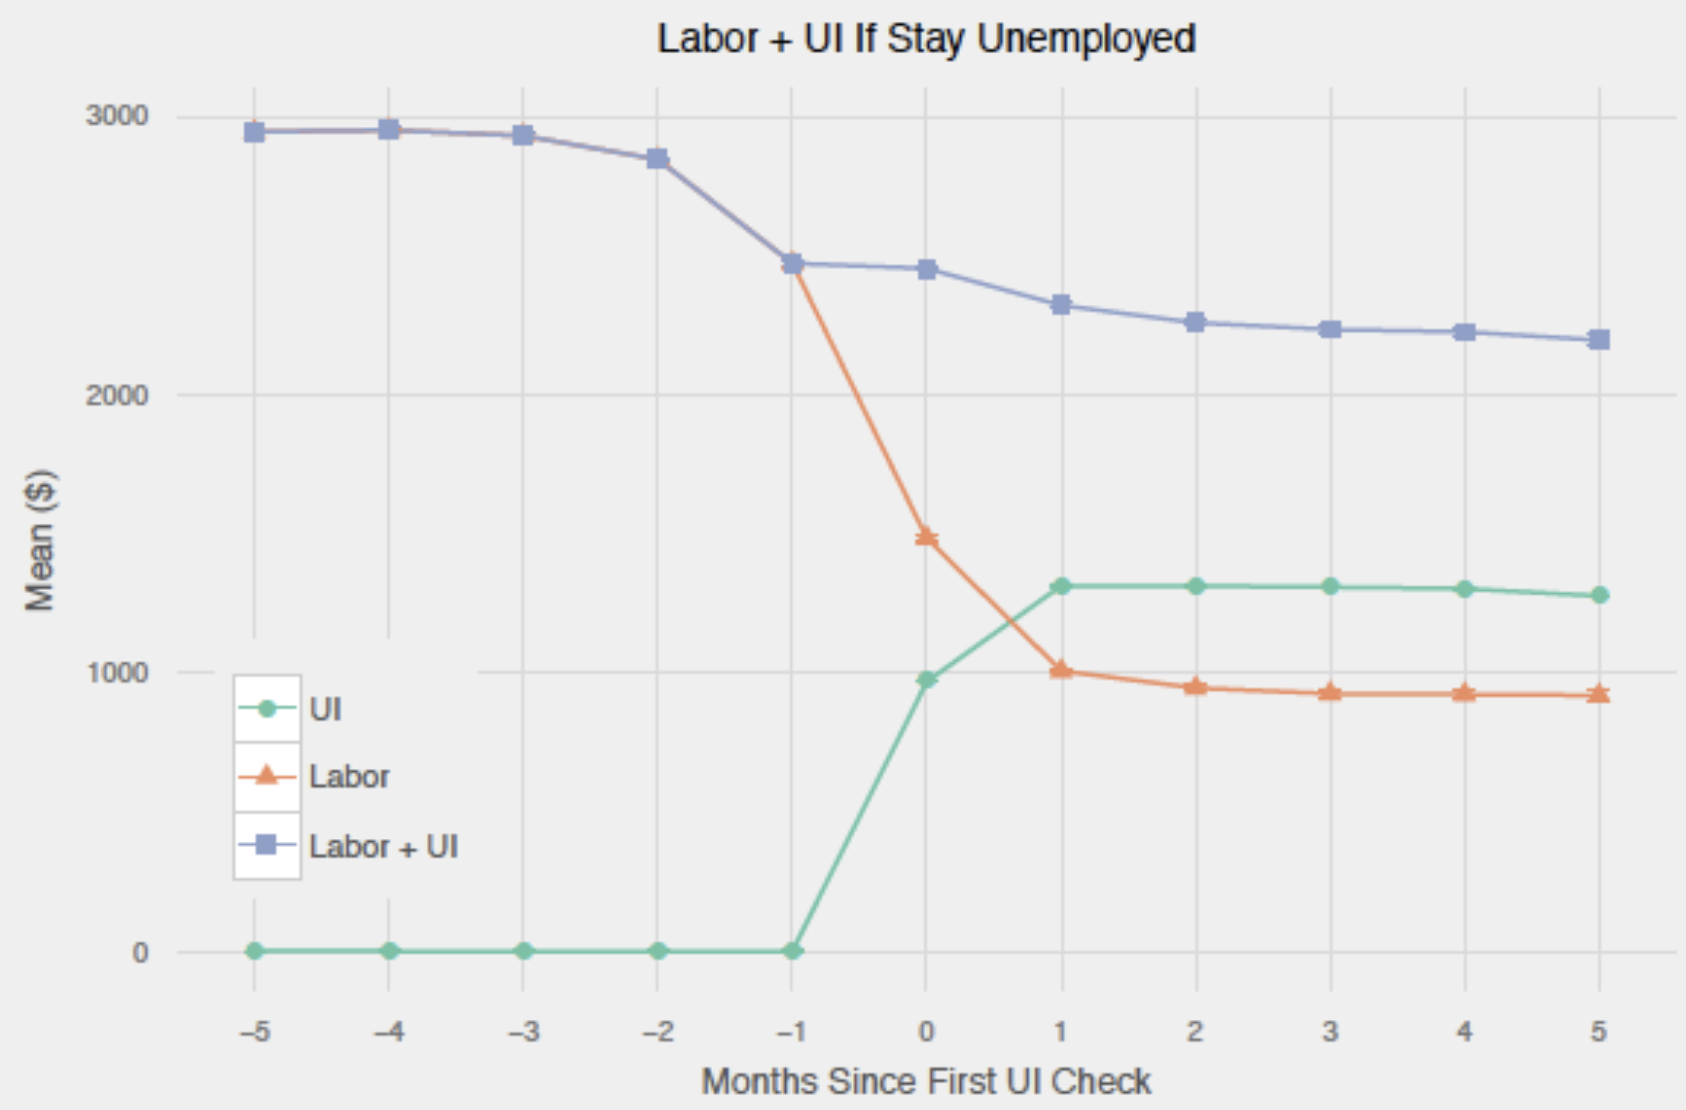
\includegraphics[width=4in]{images/ch1/Ganong_1.png}
            \caption{Labour Income and UI Benefits}
            \label{fig:Ganong_1}
        \end{figure}
        We can see a clear drop in individuals' disposable income after becoming unemployed.
        \begin{figure}[H]
            \centering
            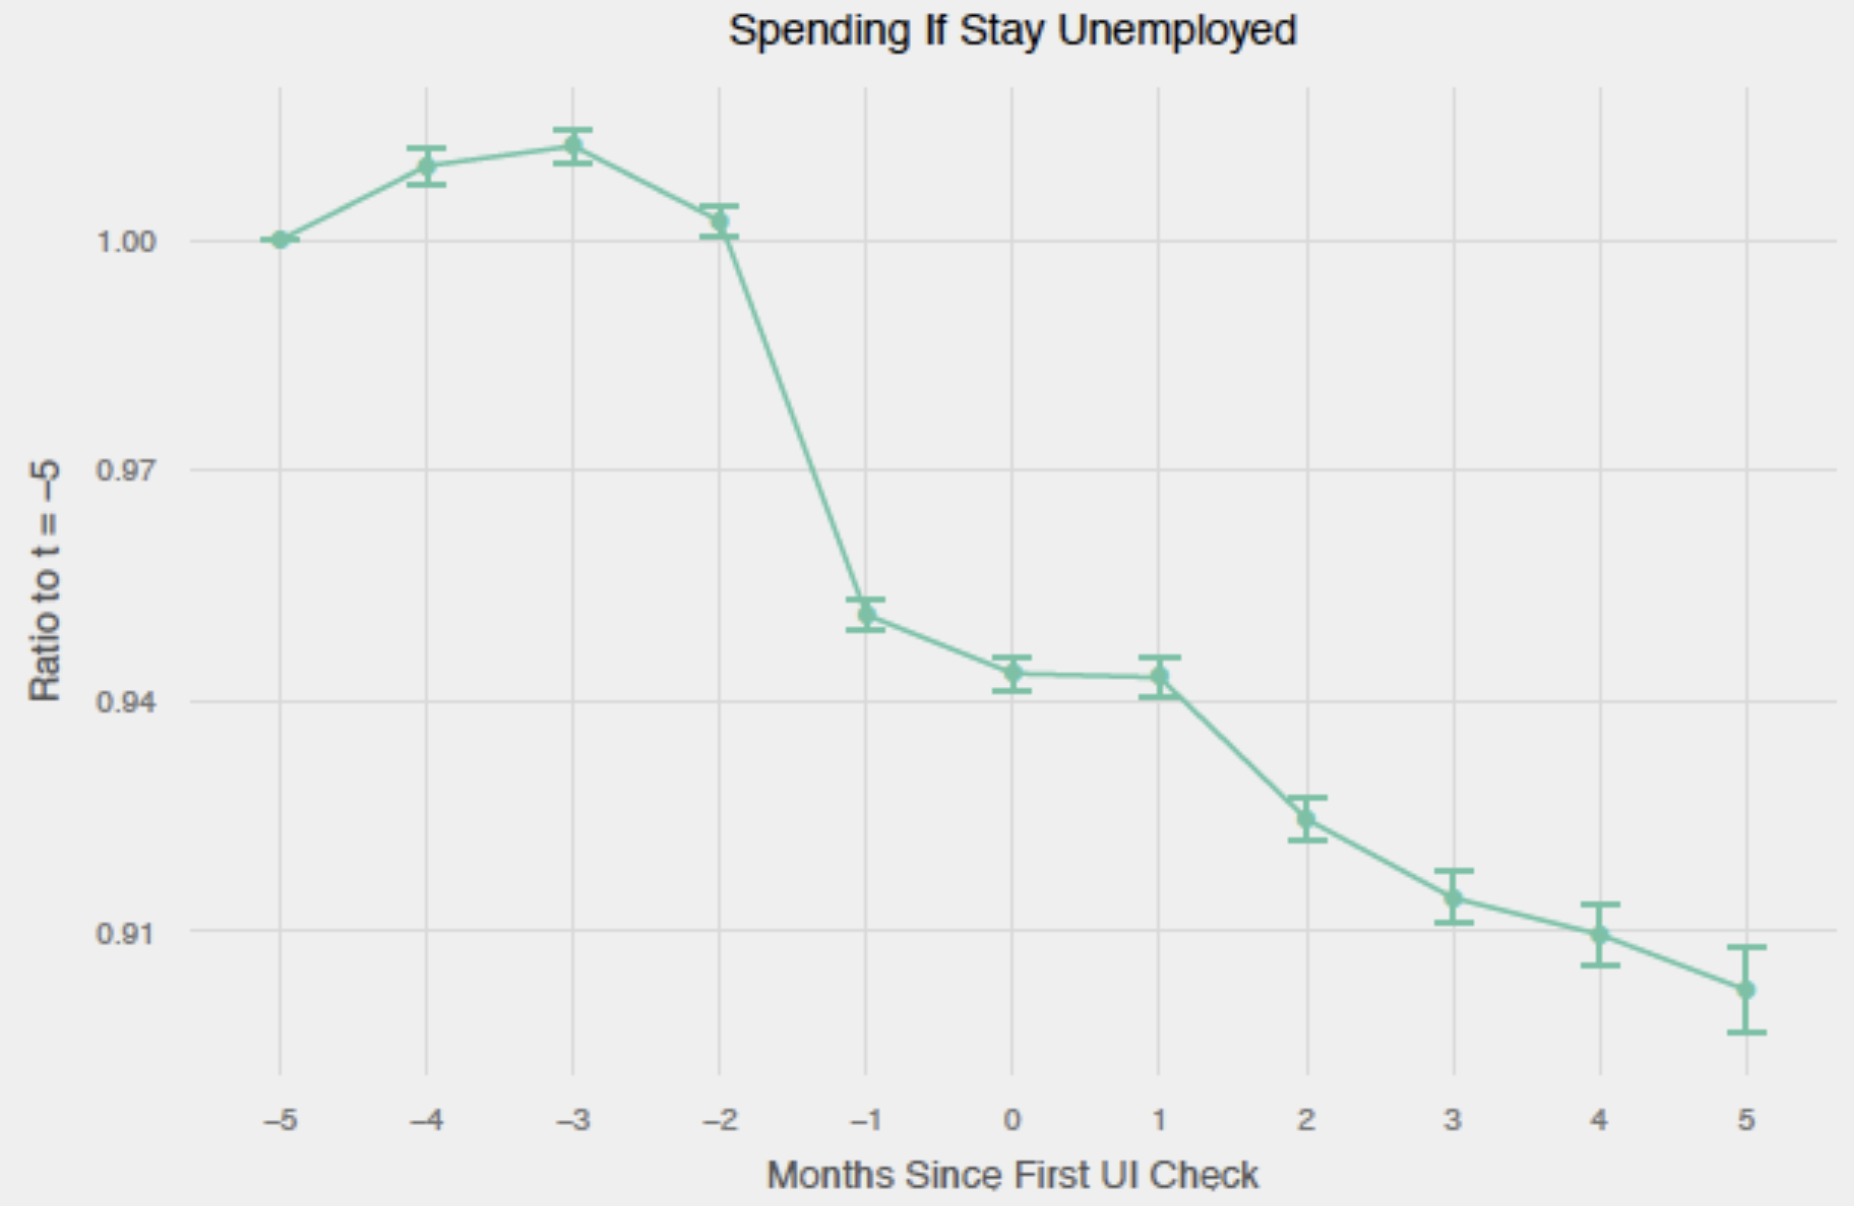
\includegraphics[width=4in]{images/ch1/Ganong_2.png}
            \caption{Spending if Individuals Stay Unemployed}
            \label{fig:Ganong_2}
        \end{figure}
        We can see that, if individuals stay unemployed, their spending will keep decreasing.
        \begin{figure}[H]
            \centering
            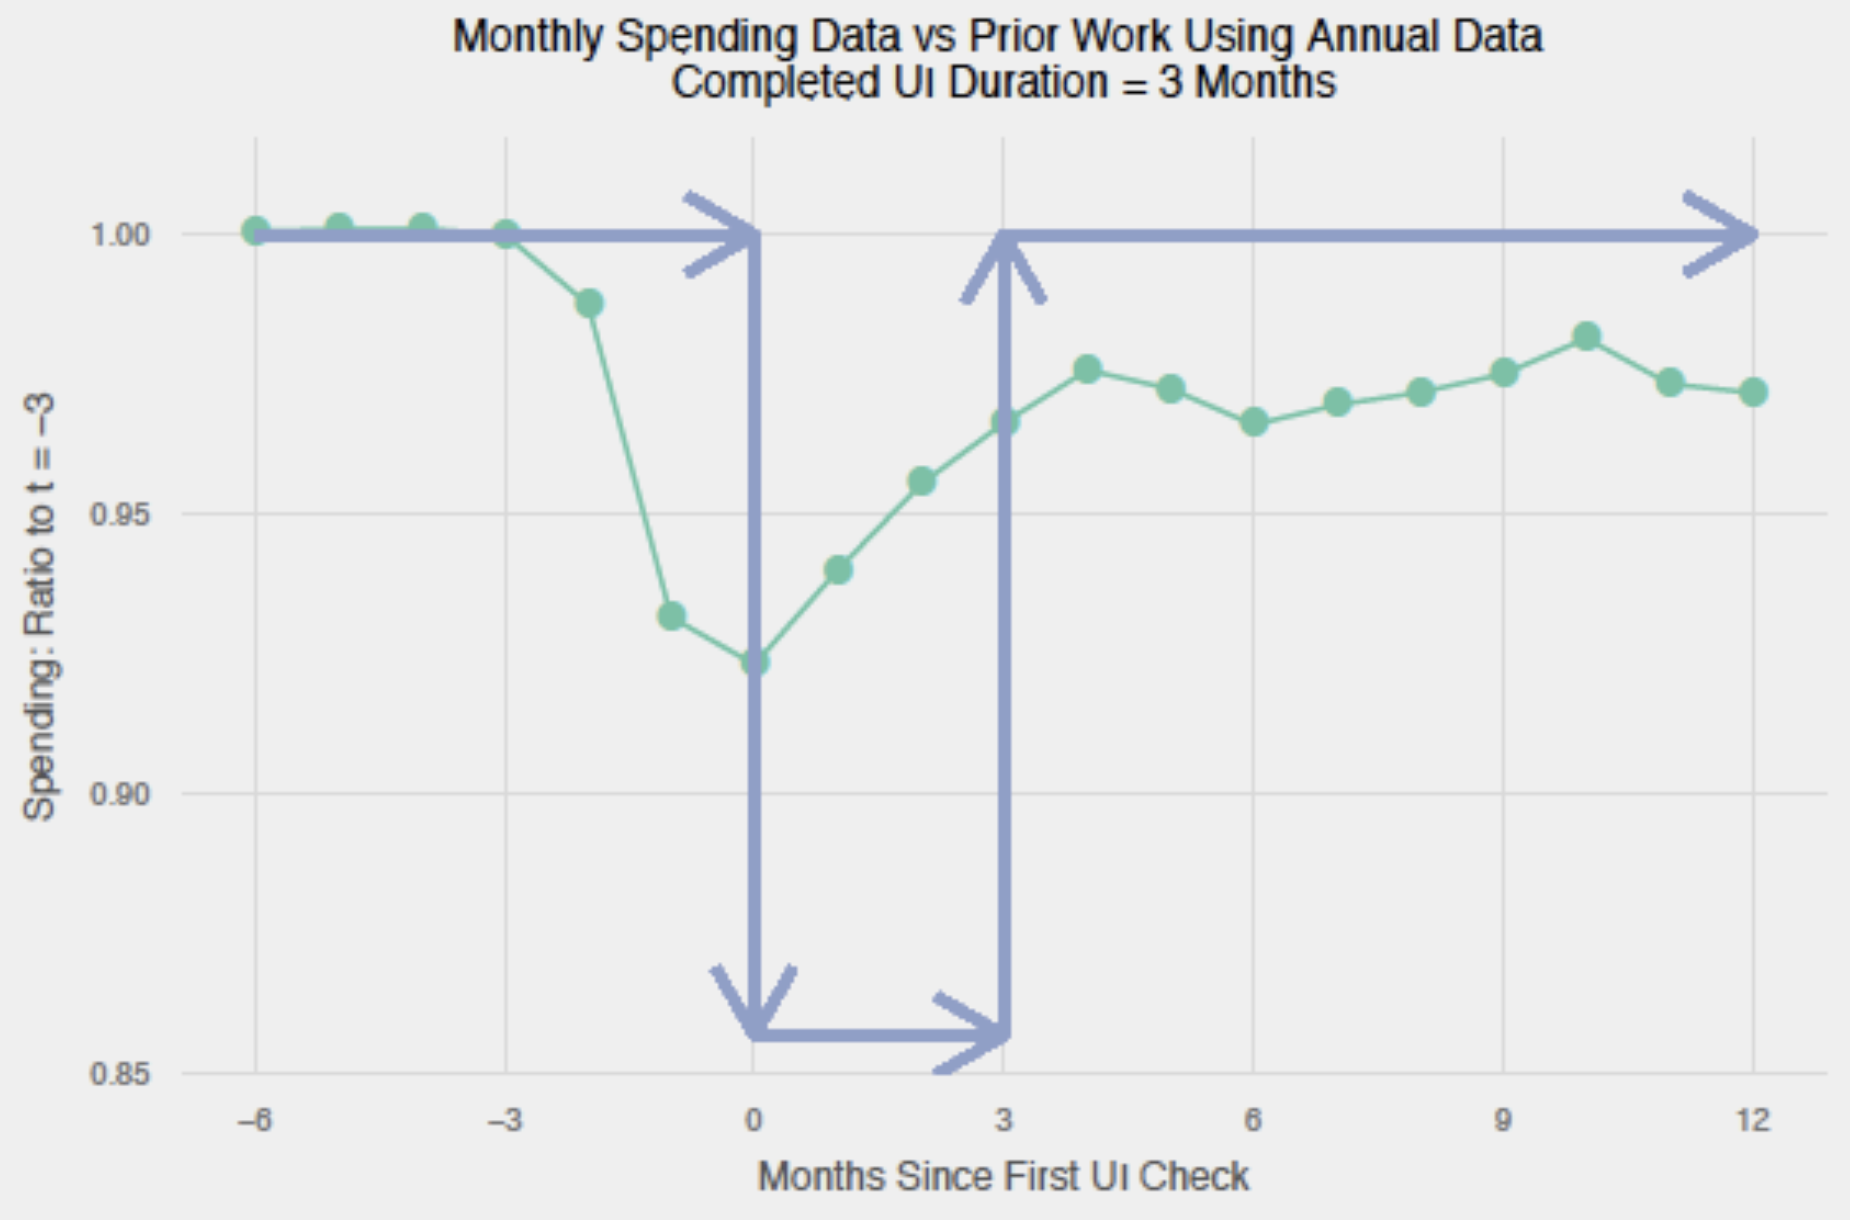
\includegraphics[width=4in]{images/ch1/Ganong_3.png}
            \caption{Spending if Individuals Find a Job after 3 Months}
            \label{fig:Ganong_3}
        \end{figure}
        However, if they find a job after 3 months, their consumption drop will be much less.
        \begin{figure}[H]
            \centering
            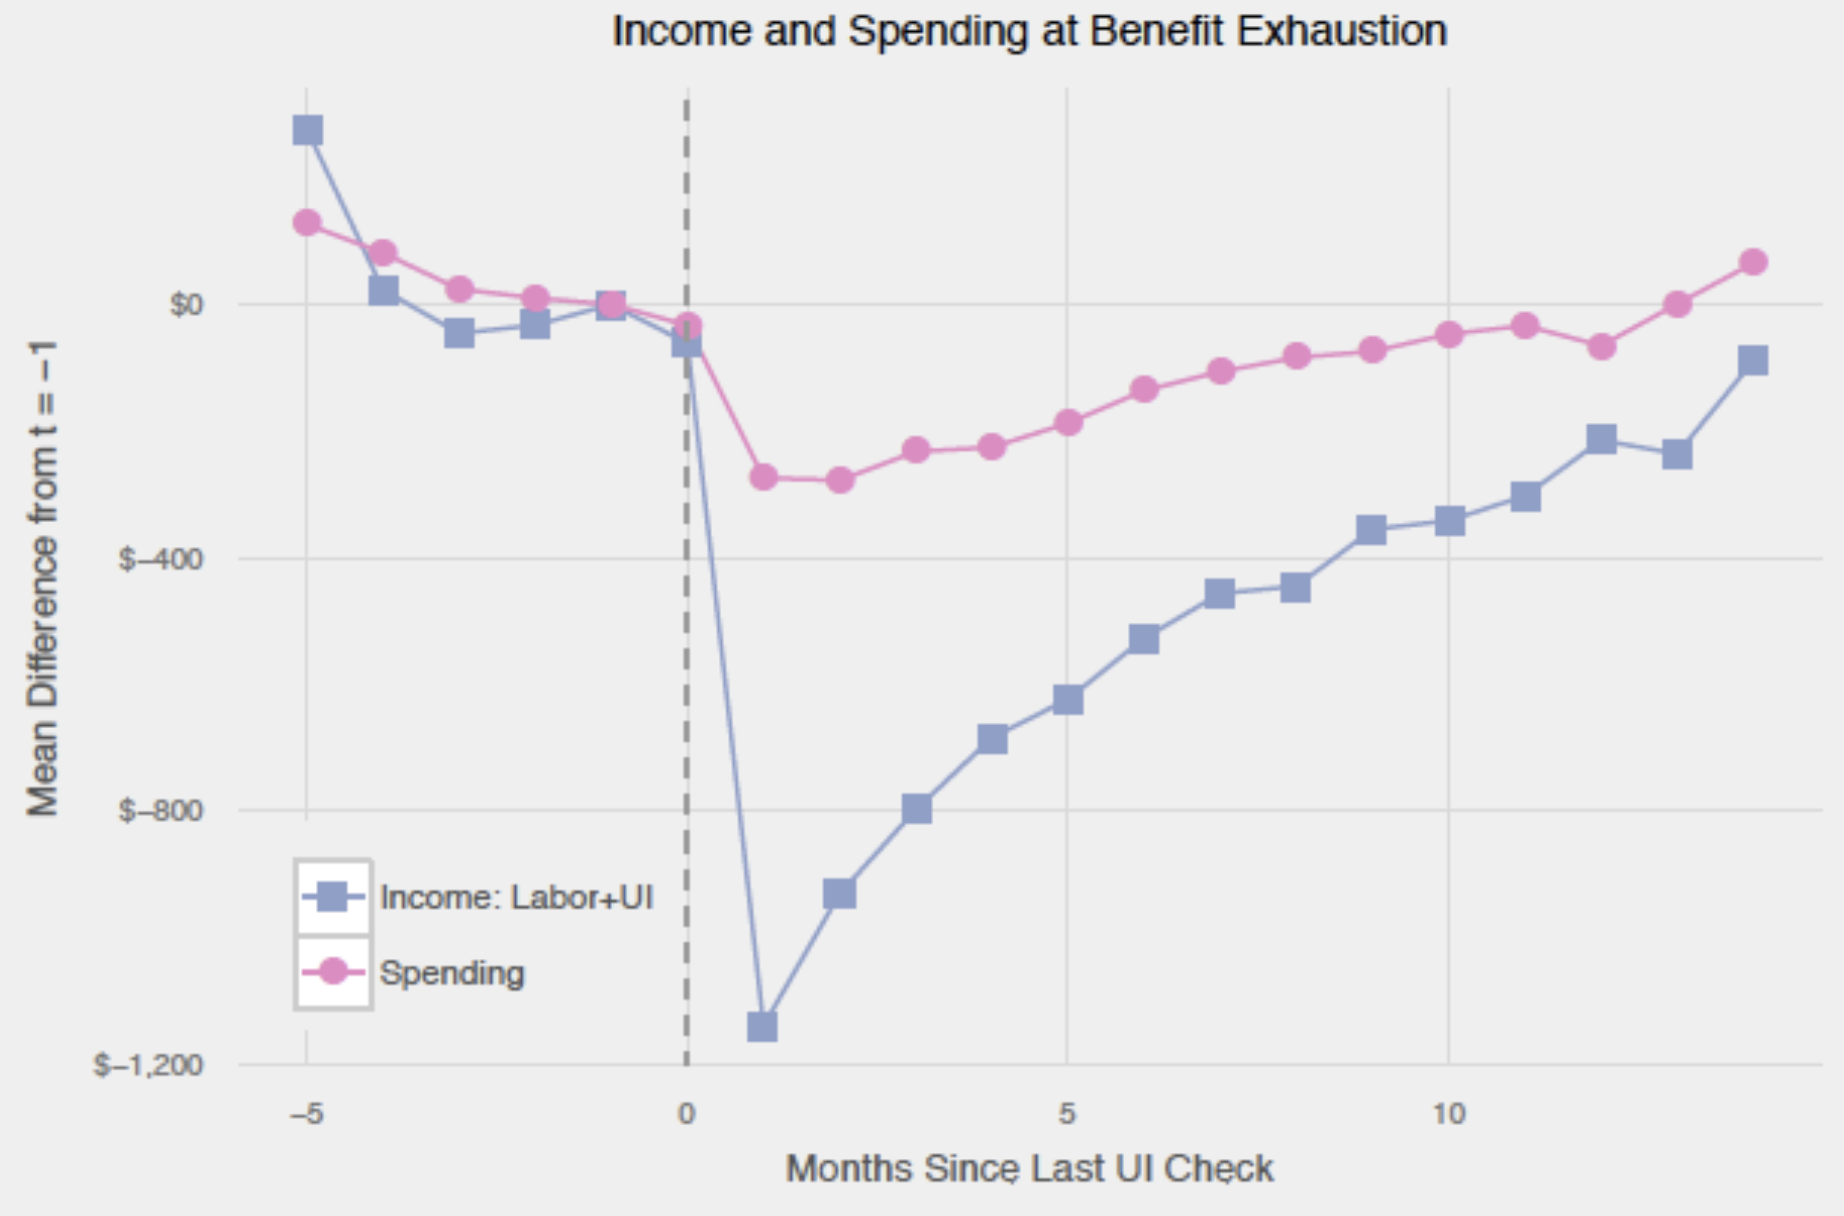
\includegraphics[width=4in]{images/ch1/Ganong_4.png}
            \caption{Consumption and Income Paths}
            \label{fig:Ganong_4}
        \end{figure}
        The figure above clearly indicates that, during unemployment, people are spending more than their income, suggesting that they are smoothing their consumption.
        
    \subsection{Using Administrative Data}
        Kolsrud, Landais, Nilsson and Spinnewijn (2016) uses administrative data on unemployment, which is linked to data on income and wealth in Sweden. They use income and wealth changes to create a registry-based consumption measure. Again, this overcomes the small sample problem present in survey data.
        \begin{figure}[H]
            \centering
            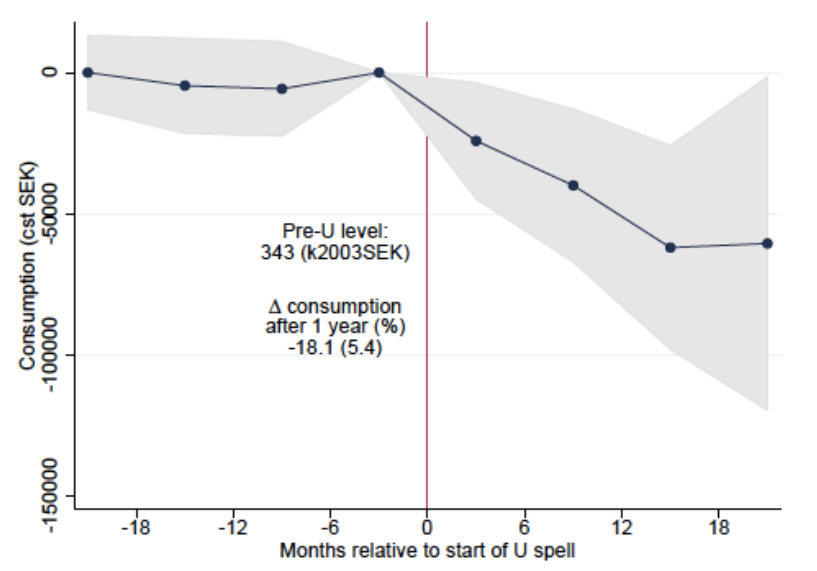
\includegraphics[width=4in]{images/ch1/Kolsrud_1.png}
            \caption{Kolsrud's Results}
            \label{fig:Kolsrudl}
        \end{figure}
        Their results also corroborated the existence of consumption smoothing.
        
\section{$\star$ Implication of the Empirical Evidence on the Optimal UI}
    
    \subsection{Is Our Current UI Benefit Optimal?}
        Recall our "sufficient statistical approach" version (equation \ref{eqn:ui_hm_sufficient}) of the Main Equation of Optimal UI:
        \begin{equation*}
        \color{red}
            \underbrace{\frac{1}{1-p}\times{\epsilon_{p,b}}}_{\text{Moral\ Hazard\ Cost}} \approx \underbrace{\gamma \times \frac{\Delta c}{c^e}}_{\text{Insurance\ Value}}
        \end{equation*}
        From our empirical researches:
        \begin{itemize}
            \item Consumption drop $\frac{\Delta c}{c^e}$ is around 10\%
            \item Elasticity of probability of unemployment with respect to UI benefit level $\epsilon_{p,b}$ is around 0.3
            \item The probability of being employed $(1-p)$ is around 90-95\%, depending on the state of the economy
            \item Survey results suggest an average RRA $\gamma$ around 2
        \end{itemize}
        Plug in those values:
        $$\underbrace{\frac{1}{0.95}\times{0.3} \approx 0.316}_{\text{Moral\ Hazard\ Cost}} > \underbrace{2 \times 0.1 = 0.2}_{\text{Insurance\ Value}}$$
        $$\text{Moral\ Hazard\ Cost} > \text{Insurance\ Value}\ \Rightarrow\ b>b^*$$
        Currently, the moral hazard cost is higher than the insurance value, indicating that our UI benefit level is too high (\emph{too generous}). We should cut the benefit level to optimize.
        
    \subsection{Counter-arguments by Chetty and Szeidl (2007): Consumption Commitment \& Risk Aversion}
        Chetty and Szeidl (2007) pointed out that risk aversion, $\gamma$, is poorly identified, and it appears to vary substantially according to specific situations. Specifically, people with consumption commitments tend to have higher risk aversion as explained below.
        \subsubsection{Consumption Commitment}
        Chetty and Szeidl extended the standard expected utility model to incorporate goods whose consumption is hard to adjust (e.g. mortgage).
        
        The standard utility model assumes that there is only one consumption good $c$, and people can cut back on all consumption goods freely anytime. This implies that, when unemployed, consumption of food, housing, cars, furniture... will all drop.
        
        However, in practice, it is hard to adjust many elements of consumption in short run due to adjustment costs.
        \begin{figure}[H]
            \centering
            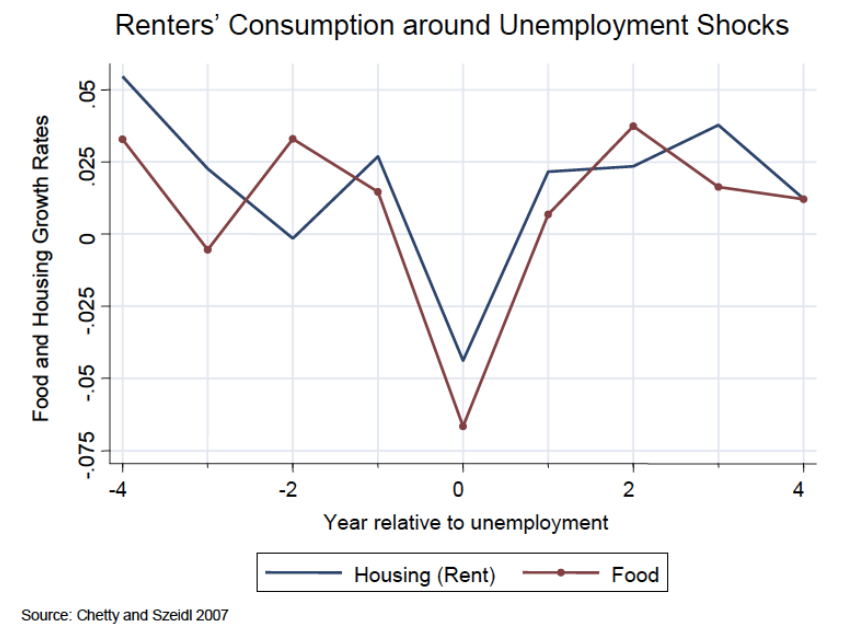
\includegraphics[width=4in]{images/ch1/Chetty_1.png}
            \caption{Consumption Commitment}
            \label{fig:Chetty}
        \end{figure}
        Shown above, compared with consumption on foods, rents are much harder to be cut off. Therefore, facing unemployment, individuals may need to reduce more flexible consumption, such as foods. In this case, the actual welfare loss will be greater.
        \subsubsection{Higher Risk Aversion}
        Chetty's model with consumption commitments suggests that risk aversion $\gamma$ may be greater than 4 when agents are hit by an unemployment shock, because consumption commitment amplifies negative utility effects, making people more dislike negative income shocks.
        
        Plugging in this value:
        $$\underbrace{\frac{1}{0.95}\times{0.3} \approx 0.316}_{\text{Moral\ Hazard\ Cost}} < \underbrace{4 \times 0.1 = 0.4}_{\text{Insurance\ Value}}$$
        $$\text{Moral\ Hazard\ Cost} < \text{Insurance\ Value}\ \Rightarrow\ b<b^*$$
        
        Therefore, under this more realistic model, our current UI benefit level is lower than the optimal level.
    
\section{Should UI Benefits Vary by the Business Cycle?}
    Our optimization requires equalization of insurance value and moral hazard cost, which contain parameters: $p, \epsilon_{p,b}, \frac{\Delta c}{c^e}, \gamma$. If they vary with the business cycle, our optimal UI benefits should adjust accordingly. Thus, again, this is an empirical question.
    
    \subsection{Unemployment Duration and the Business Cycle}
        Schmieder, von Wachter and Bender (2011) conclude that, during recessions:
        \begin{itemize}
            \item the responsiveness of unemployment duration to an additional month of UI benefit is lower. ($\frac{dp}{db}$ is lower)
            \item the probability of employment is lower ($p$ is lower) 
        \end{itemize}
        Therefore, the \empha{elasticity of unemployment rate with respect to benefits $\epsilon_{p,b}$ is lower in recessions}. This in turn indicates lower moral hazard costs, and UI benefits should be higher in recessions to optimise.
        \begin{figure}[H]
            \centering
            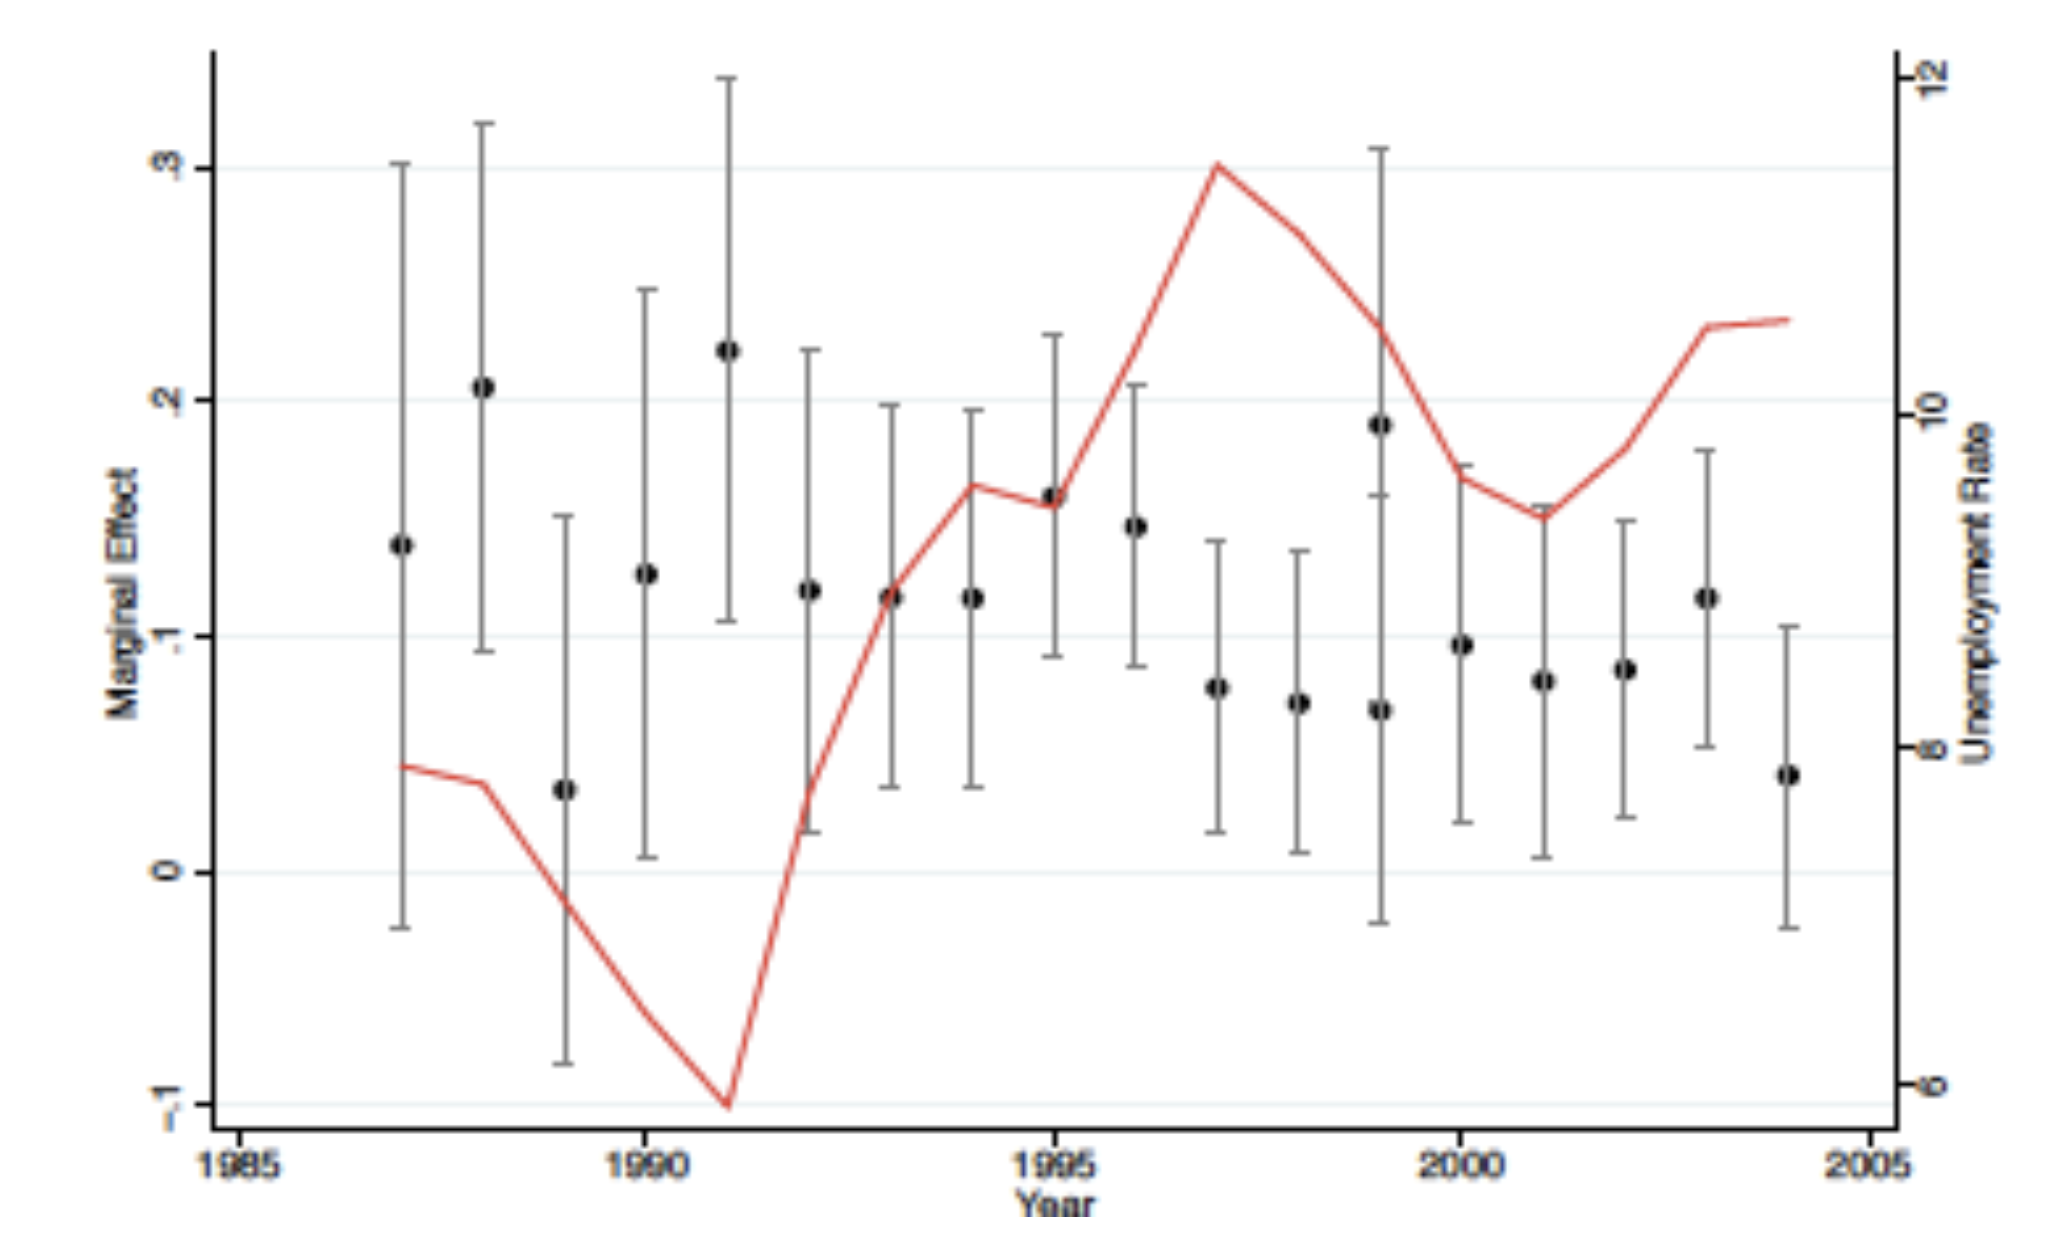
\includegraphics[width=4in]{images/ch1/Schmieder.png}
            \caption{Red line: unemployment rate; Marginal effect: shows $\frac{dp}{db}$}
        \end{figure}
        
    \subsection{Consumption Smoothing and the Business Cycle}
    Kroft and Notowigdio (2015) replicate and extend works by Gruber (1997). They estimate how the effect of UI on the consumption drop upon unemployment varies with the state unemployment rate in the previous year. They do not find evidence for larger or smaller drop in consumption when unemployment is higher. Thus, we can conclude that the \empha{value of consumption smoothing does not vary with the business cycle}.
    
    \subsection{Counter-cyclical UI Benefits}
    As discussed in the two subsections above: during a recession, moral hazard costs decrease while insurance values do not change. Therefore, it is \empha{optimal to implement a counter-cyclical UI benefit scheme}: benefits should be larger in recessions and lower in booms.
    
\section{Extension: Match Quality and Long-term Effects}
    We ignored another potential benefit of UI schemes in our simple model above: \emphb{improvements in match quality}. When people become unemployed and face the pressure of purchasing necessities, they may be forced to take worse jobs. For example, an experienced engineer may have no choice but to work in McDonald's. Provision of UI benefits may alleviate such mismatching.
    
    On the other hand, if UI benefits induce people to stay unemployed longer, there may be \emphb{skill deprecation}: an unemployed individual may lose his/her social skills and self-esteem.
    
    Which of these dominates is an empirical question:
    \begin{itemize}
        \item Card, Chetty, and Weber (2007) exploit the same discontinuity in Austria to examine the effect on subsequent wages or on subsequent job tenure, and found no significant improvement
        \item Schmieder et al. (2015) use RDD to examine the effect of extending UI eligibility from 12 months to 18 months at age 42 in Germany. They found non-employment duration increases by 1 months while re-employment wage decrease by 3\%, supporting skill deprecation.
        \item Nekoei and Weber (2015) use RDD to examine the effect of extending UI eligibility from 7.5 months to 9.5 months at age 42 in Austria. They find that non-employment duration increases by 3 days, and they also find positive effects on wages, suggesting that UI benefits improve matching quality.
    \end{itemize}
    
    All in all, empirical results are contradictory. In reality, it is \empha{very likely that both match quality improvement and skill depreciation exist}. The overall effect depends on which one dominates.